\section{Experiments and results}\label{sec:experiments}

\begin{table}
  \caption{\acs*{auc} of the individual features for each method.}
  \centering
  \begin{tabular}{l c c}
    \toprule
    \textbf{Features} & Un-normalized data & Normalized data \\
    \midrule
    \textbf{Brix model} & & \\
    \quad $A$         & & \\
    \quad $k_{el}$    & & \\
    \quad $k_{ep}$    & & \\
    \textbf{Hoffmann model} & & \\
    \quad $A$         & & \\
    \quad $k_{el}$    & & \\
    \quad $k_{ep}$    & & \\
    \textbf{Tofts model with population \ac{aif}} & & \\
    \quad $K_{trans}$ & & \\
    \quad $v_{p}$     & & \\
    \quad $k_{ep}$    & & \\
    \textbf{Tofts model with patient \ac{aif}} & & \\
    \quad $K_{trans}$ & & \\
    \quad $v_{p}$     & & \\
    \quad $k_{ep}$    & & \\
    \textbf{\ac{pun} model} & & \\
    \quad $a_0$       & & \\
    \quad $r$         & & \\
    \quad $\beta$     & & \\
    \textbf{Semi-quantitative analysis} & & \\
    \quad wash-in     & & \\
    \quad wash-out    & & \\
    \quad IAUC        & & \\
    \quad $\tau$      & & \\
    \quad $S_M - S_0$ & & \\
    \bottomrule
  \end{tabular}
  \label{tab:resfeats}
\end{table}

\begin{figure}
  \centering
  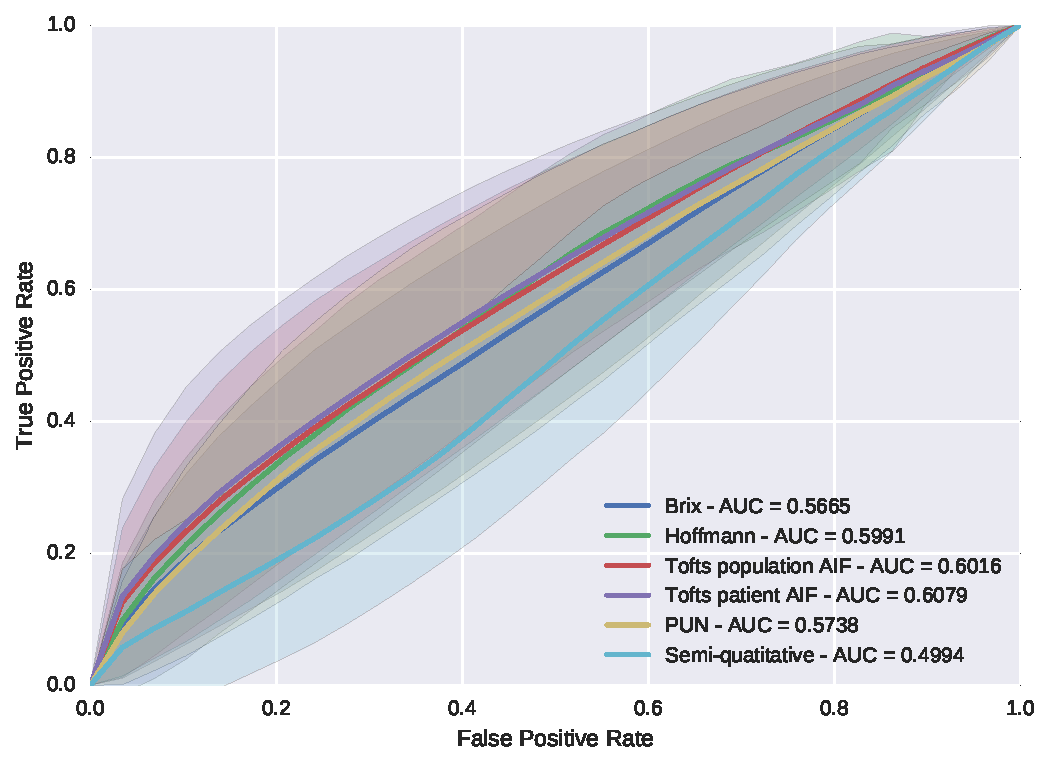
\includegraphics[width=0.7\linewidth]{03_experiments/figures/unormalized/rf.pdf}
  \caption{\acs*{roc} analysis using a \acs*{rf} classifier for the different quantification methods without data normalization.}
  \label{fig:rfunorm}
\end{figure}

\begin{figure}
  \centering
  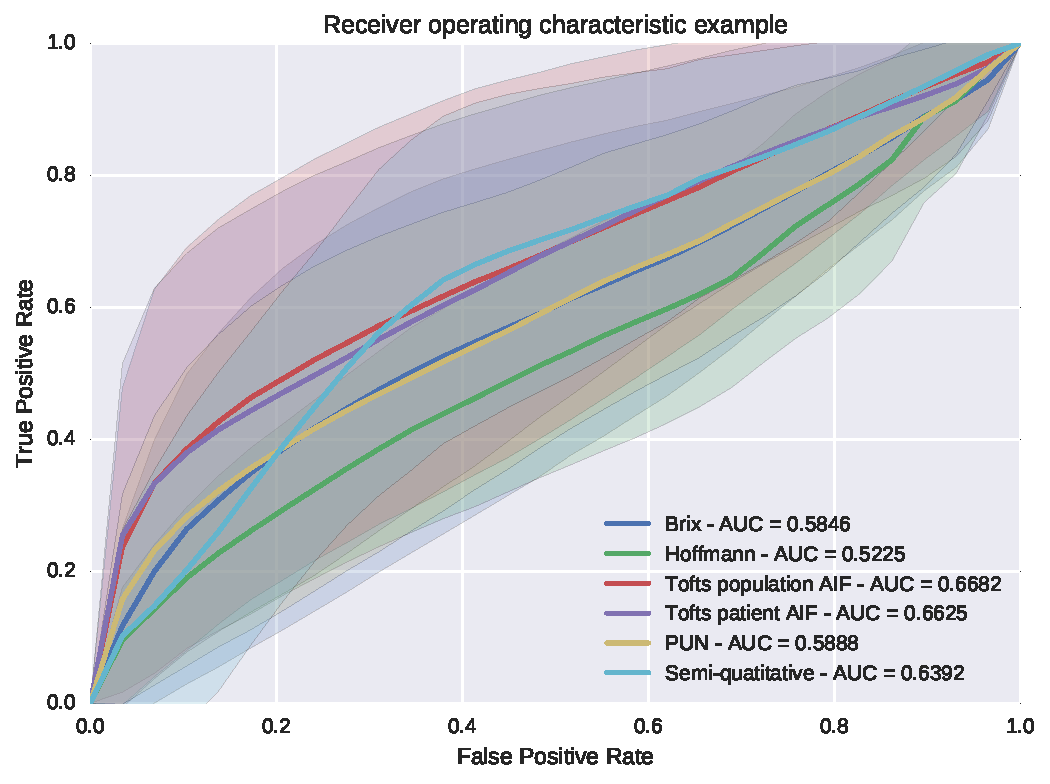
\includegraphics[width=0.7\linewidth]{03_experiments/figures/unormalized/nb.pdf}
  \caption{\acs*{roc} analysis using a \acs*{nb} classifier for the different quantification methods without data normalization.}
  \label{fig:rfunorm}
\end{figure}

\begin{figure}
  \centering
  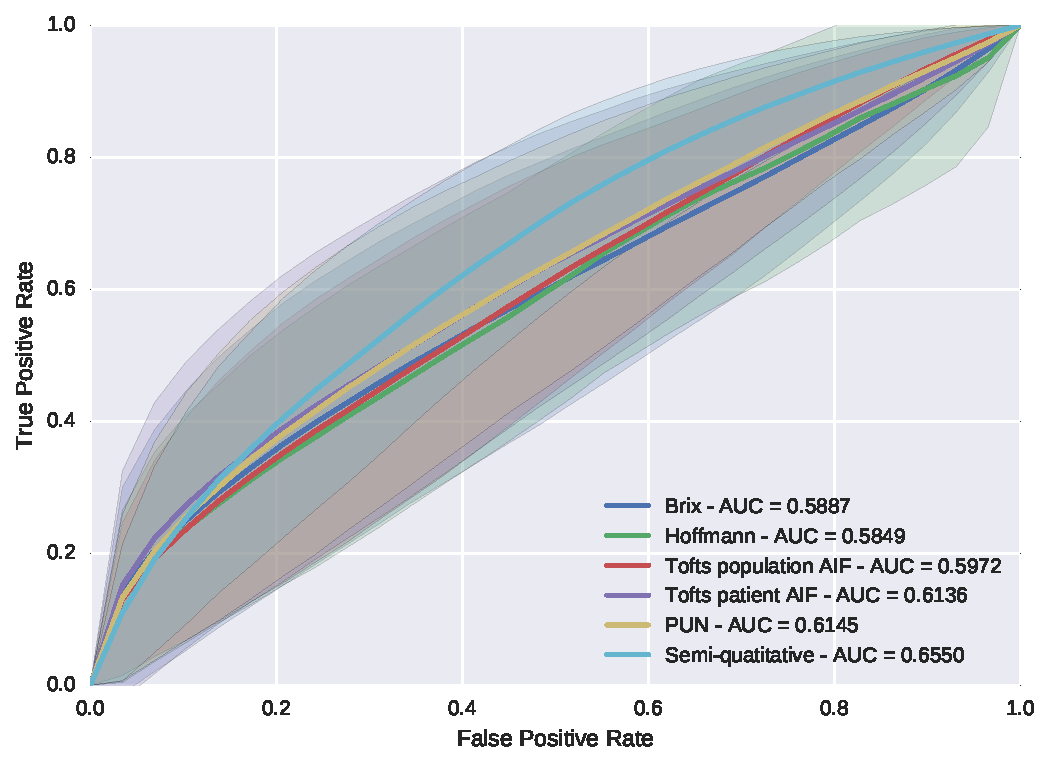
\includegraphics[width=0.7\linewidth]{03_experiments/figures/normalized/rf.pdf}
  \caption{\acs*{roc} analysis using a \acs*{rf} classifier for the different quantification methods with data normalization.}
  \label{fig:rfunorm}
\end{figure}

\begin{figure}
  \centering
  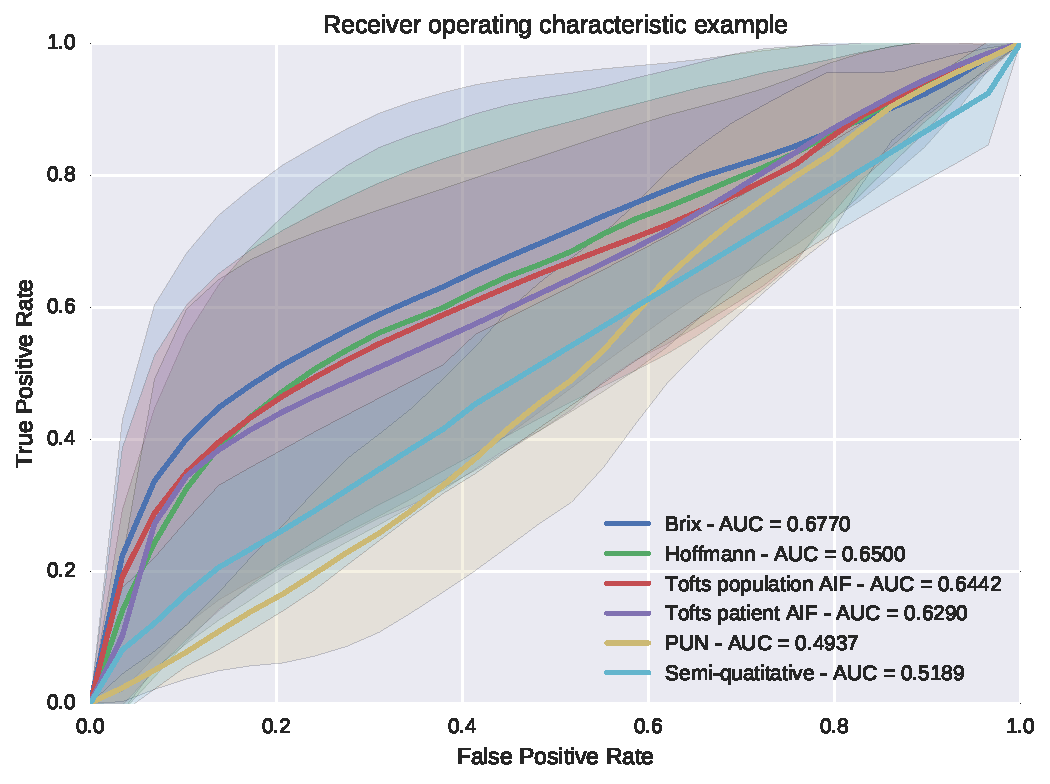
\includegraphics[width=0.7\linewidth]{03_experiments/figures/normalized/nb.pdf}
  \caption{\acs*{roc} analysis using a \acs*{nb} classifier for the different quantification methods with data normalization.}
  \label{fig:rfunorm}
\end{figure}

%%% Local Variables: 
%%% mode: latex
%%% TeX-master: "../main"
%%% End: 
